\chapter{Diseño}

El proyecto tiene dos partes claramente diferenciadas a la hora de plantear el diseño:

\begin{itemize}
  \item \textbf{Diseño de clases.}
  \item \textbf{Diseño de las interfaces de usuario.}
  \item \textbf{Mecanismo de adición de vistas.}
\end{itemize}

Además, hay que tener en cuenta que uno de los objetivos principales es que la aplicación sea facilmente extensible y que permita añadir nuevas interfaces de usuario para propiedades y dispositivos por lo que es parte importante de la fase de diseño, en la que se describirán todos detalladamente.

\bigskip
\section{Diseño de clases}

En todo proyecto de software es muy importante diseñar correctamente las clases antes de comenzar la fase de implementación. Un mal diseño puede provocar retrasos en la fase de implementación, incluso obligando a retroceder y rediseñarlas.

\bigskip
Podemos dividir el diseño en cuatro bloques:

\begin{itemize}
  \item \textbf{Diseño de las actividades de Android.}
  \item \textbf{Diseño del cliente INDI.}
  \item \textbf{Diseño de las clases manejadoras de propiedades.}
  \item \textbf{Diseño de las clases manejadoras de dispositivos.}
\end{itemize}

\newpage
\subsection{Diseño de las actividades de Android}

Las actividades en android son el cuerpo principal de las aplicaciónes. Son ejecutadas en la hebra principal del sistema y gestionan la interfaz principal. Se pueden tener tantas actividades como se desee. En nuestro caso tenemos dos actividades:


\begin{itemize}
  \item \textbf{Front activity}
  \item \textbf{Main activity}
\end{itemize}

\subsubsection{Front activity}

Esta actividad inicia la aplicación, mostrando una pantalla de inicio con la información como portada. Una vez lanzada la aplicación esta actividad no volvera a ejecutarse a no ser que el sistema cierre la aplicación o que lo haga el usuario explicitamente. Como podemos ver en el diagrama de la figura \ref{fig:diag_front}, la actividad solo tiene una clase que hereda de \textit{AppCompatActivity}. Esta clase pertenece a la biblioteca de compatibilidad de \textbf{android}. Además, esta actividad tiene un objeto de la clase \textit{UpdateProgress}. Esta clase sirve para ejecutar código en una hebra separada en la que controlar el progreso.

\bigskip
\begin{figure}[!ht]
  \begin{center}
  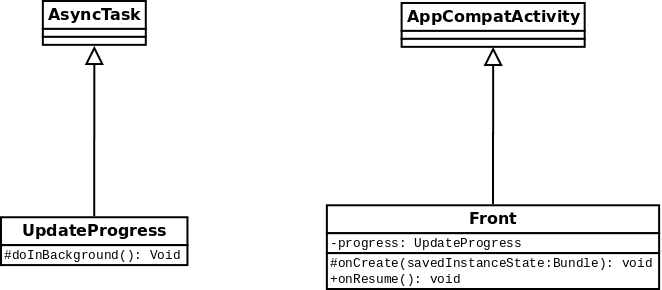
\includegraphics[width=1\textwidth]{../images/front_diag.png}
  \caption{Diagrama de clases de la actividad front}
  \label{fig:diag_front}
  \end{center}
\end{figure}


\subsubsection{Main activity}

La actividad principal es el núcleo de la aplicación. Esta clase es la más importante ya que su ciclo de vida condiciona el ciclo de vida de la aplicación. Es por ello que esta clase es la más compleja. En la figura \ref{fig:diag_main_activity} podemos ver el diagrama de clases. Las clases que no contienen ninguna especificación pertenecen a \textbf{Android} y simplemente se añaden para indicar las relaciones que las clases implementadas.

\bigskip
Dado que esta clase es la responsable de la visualización de los distintos menús, necesitamos declarar objetos de las clases que representan cada uno de los elementos visuales principales, tales como \textit{NavigationView} o \textit{TabLayout}.

\bigskip
Por otro lado, la actividad implementa una serie de escuchadores que le permiten capturar los eventos disparados por los distintos botones de la interfaz de usuario para realizar las acciones oportunas.

\bigskip
Además de estas clases, se ha diseñado la clase \textit{Settings} que representa las configuraciones generales de la aplicacion: notificaciones y carpeta por defecto.

\bigskip
En el diagrama también podemos ver la clase \textit{Connection}. Esta clase representa las conexiones con el servidor y es por ella que se describen en el apartado correspondiente.


\bigskip
\begin{figure}[!ht]
  \begin{center}
  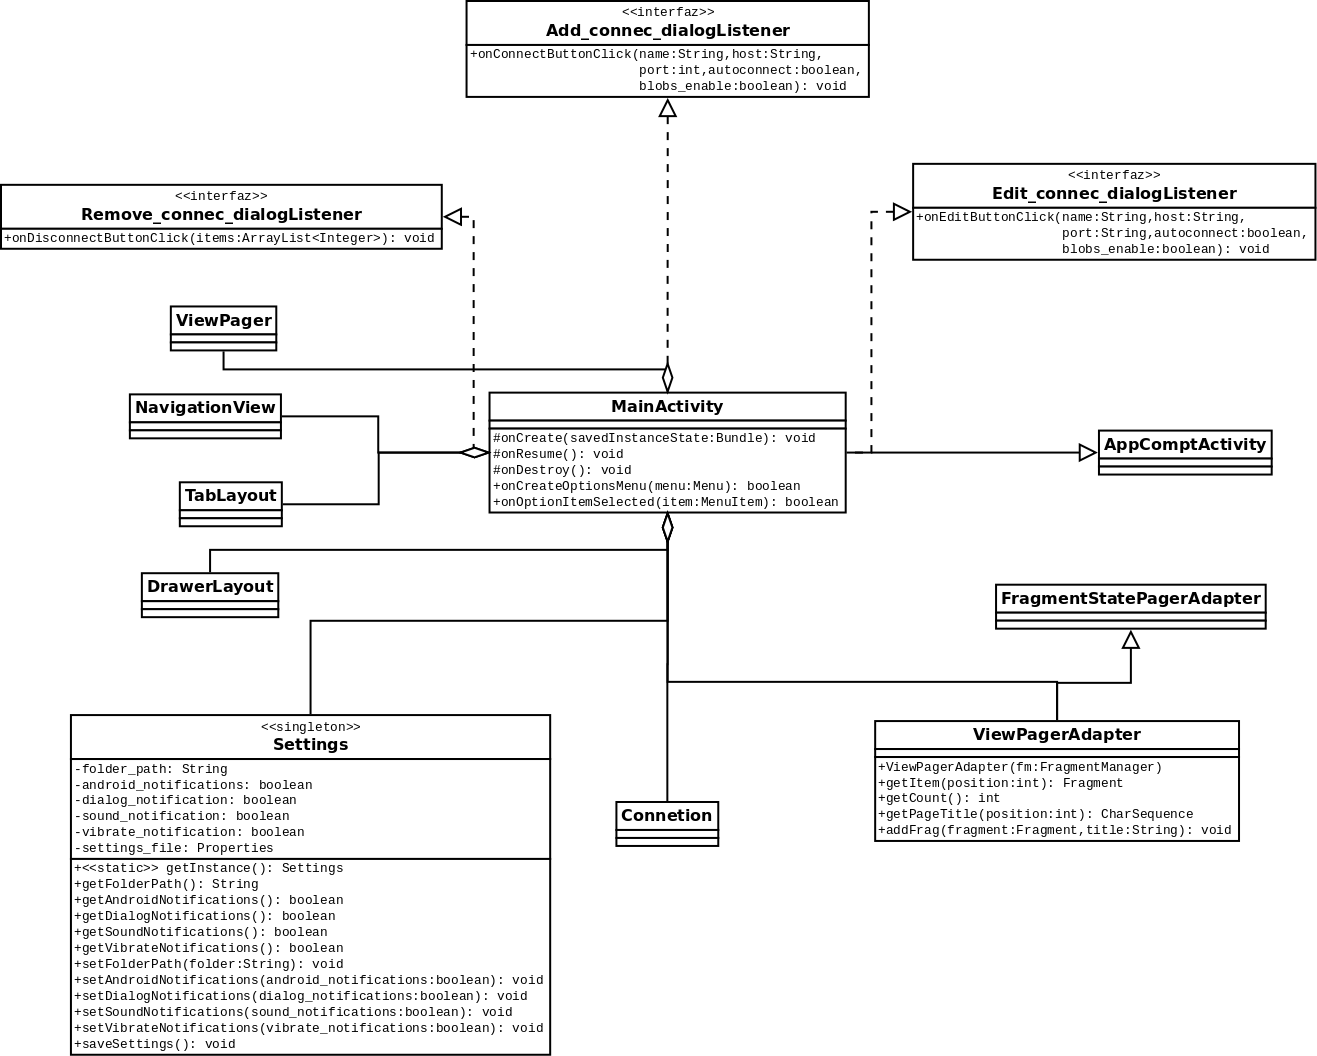
\includegraphics[width=1\textwidth]{../images/main_activity.png}
  \caption{Diagrama de clases de la actividad principal}
  \label{fig:diag_main_activity}
  \end{center}
\end{figure}


\newpage
\subsection{Diseño del cliente INDI}

La aplicación se basa en integrar la biblioteca \textbf{``INDI for Java''} para poder crear un cliente que nos permita conectarnos a cualquier servidor. Las conexiones se hacen creando conexiones tcp/ip a través de la red. \textbf{Android} establece unas restricciones muy fuertes respecto a la apertura y cierre de \textit{sockets} de red. Dado que la aruitectura del sistema esta basada en una única hebra principal que gestiona la interfaz de usuario, si iniciamos algún proceso que pueda bloquear dicha hebra, bloquearíamos todo el sistema. Por ello cualquier proceso de comunicación debe ejecutarse en una hebra secundaría. Además solo se pueden ejecutar acciones sobre la interfaz en la hebra principal.

\bigskip
Con estas restricciones, el primer paso necesario es extraer todo el código relativo a las conexiones a una hebra por conexión. Para ello se ha diseñado la clase \textit{Connection}. El objetivo principal de esta clase es lanzar en una hebra la apertura de la conexión y el intercambio de información con el servidor. Pero para poder utilizar esa información y mostrarla en pantalla necesitamos ejecutar en la hebra principal dichas acciones. 

\bigskip
\textbf{Android} nos facilita una clase para resolver este problema, aparentemente sin solución. La clase \textit{AsyncTask} tiene la peculiaridad de permtir ejecutar código en una hebra a parte y a la vez enviar información a la hebra principal para gestionarla adecuadamente. Por ello la clase \textit{Connection} lanza una hebra pero almacena en sus atributos el resultado de la consexión al servidor, permitiendo a la actividad principal procesar esos datos y mostrarlos adecuadamente. La actividad principal tendrá tantos objetos \textit{Connection} como conexiones se hayan añadido en la interfaz de usuario. Cada objeto \textit{Connection} creará una cliente INDI que le enviará todos los dispositivos y atributos que tenga y le irá informando de cualquier cambio para que estos se reflejen en la interfaz de usuario. Todas estas hebras se lanzan en paralelo, de forma que no relenticen las acciones en la interfaz de usuario.

\bigskip
Por otra parte, para que todo funcione debemos diseñar una clase cliente \textbf{INDI} para crear la conexión, y escuchar cualquier cambio en propiedades, dispositivos o en la propia conexión. Por ello esta clase implementa las tres interfaces de \textbf{INDI}

\bigskip
Para facilitar el diseño, también se ha creado una clase \textit{device}. Esta clase se útiliza para procesar las propiedades de un dispositivo \textbf{INDI}. Cada propiedad pertenece a un grupo pero a priori no puedes conocer que grupos hay. Además las propiedades no llegan según un orden por lo que hay que comprobar por cada una a que grupo pertenece, si el grupo existe ya o si hay que crearlo. De la misma forma, cuando se borra una propiedad hay que comprobar si era la última de su grupo, en cuyo caso habrá que borrarlo. La clase \textit{device} facilita estas operaciones, añadiendo una capa de abstracción más para poder obtener las propiedades organizadas y listas para ser mostradas en la interfaz de usuario.

\bigskip
Finalmente, necesitamos representar la lista de propiedades y dispositivos. Para ello usamos las \textit{listas explandilbes de Android}. Estas listas nos permiten tener dos niveles. En el primer nivel mostramos los grupos y en el segundo los elementos. Internamente tenemos una lista o \textit{adaptador} de propiedades que añadimos a la clase \textit{PropertyArrayAdapter}. Cada objeto de esta clase representa un dispositivo con todas sus propiedades. 

\bigskip
En este punto cabe destacar que podemos tener propiedades ocultas. Dichas propiedades no deben ser añadidas al adaptador, ya que todos los elementos de este son mostrados. para controlarlo, la clase \textit{Connection} es la encargada de construir los \textit{adaptadores} a partir de la información del objeto de la clase \textit{IndiClient}. Por ello en la clase \textit{Connetion} gestionamos las propiedades que estan ocultas para no agregarlas al \textit{adaptador} que le corresponda.


\bigskip
\begin{figure}[!ht]
  \begin{center}
  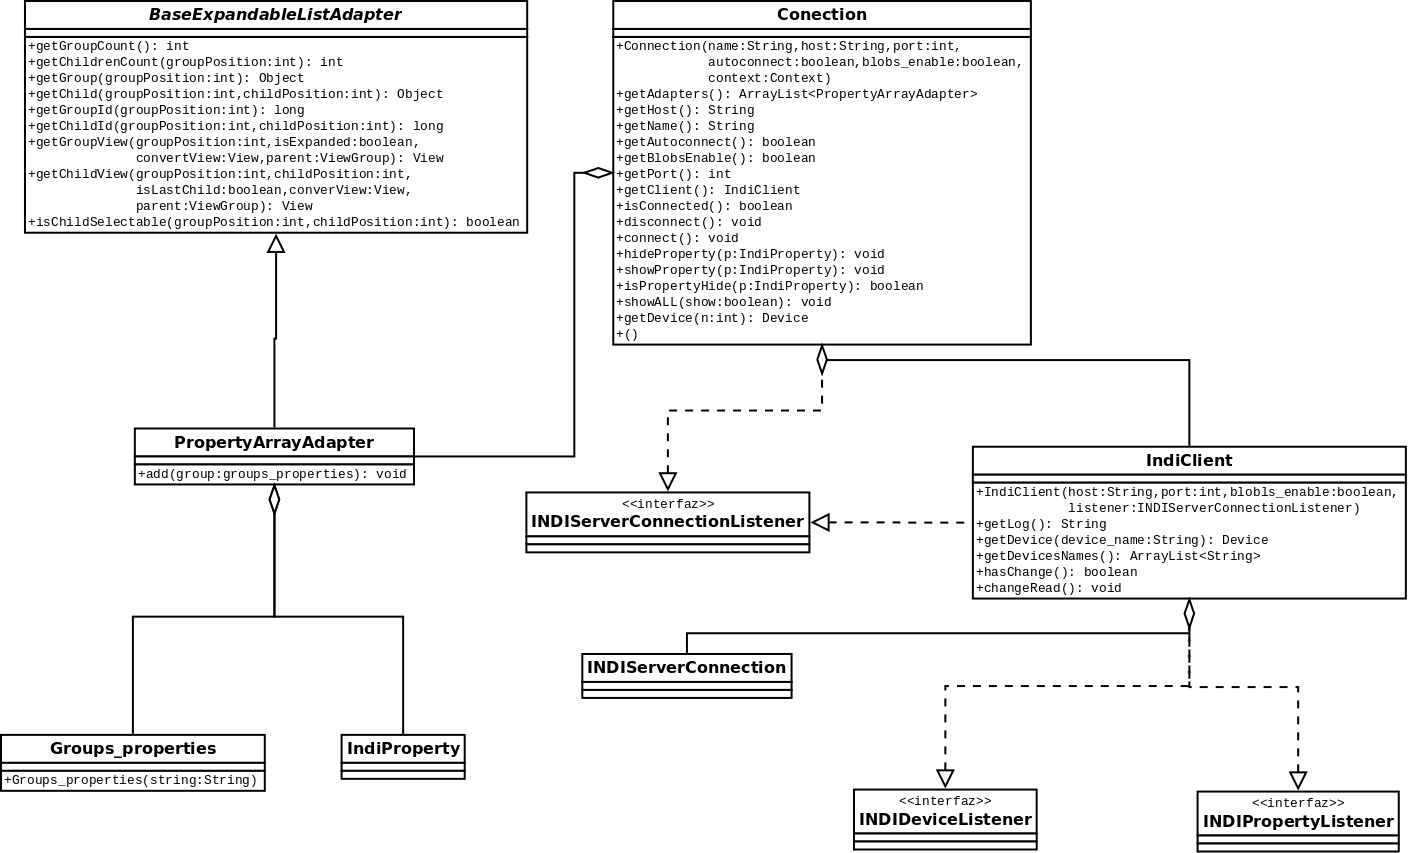
\includegraphics[width=1\textwidth]{../images/indi_diag_clases.png}
  \caption{Diagrama de clases asociadas a INDI}
  \label{fig:diag_indi_clases}
  \end{center}
\end{figure}


\newpage
\subsection{Diseño de las clases manejadoras de propiedades}

Como se explicó en la introducción, \textbf{INDI} maneja 5 tipos de porpiedades:


\begin{itemize}
  \item \textbf{Text.}
  \item \textbf{Number.}
  \item \textbf{Switch.}
  \item \textbf{Blob.}
  \item \textbf{Light.}
\end{itemize}

\bigskip
Para manejar cada una de estas propiedades se crea una clase que recibirá un objeto \textit{INDIProperty} (del que heredan todos los tipos) y según el tipo informarán de que pueden manejar dicha propiedad y construirán las interfaces de usuario para mostrarla y editarla.

\bigskip
Gracias a la creación de la interfaz de Java \textit{UIPropertyManager} podemos añadir más manejadores de propiedades. Para ilustrar su uso se han creado dos manejadores más:

\begin{itemize}
  \item \textbf{Connection.}
  \item \textbf{Abort.}
\end{itemize}

\bigskip
Estas dos propiedades son de tipo \textit{Switch} pero tienen la peculiaridad de que siempre tienen la misma estructura: mismo número de elementos, mismo nombre para cada elemento, etc. Por ello podemos analizar la propiedad recibida y ver si es de esos tipos, informando de que podemos manejarla, y construyendo vistas especificas para esas propiedades (como son de tipo \textit{Switch} su vista por defecto sería la de todas las propiedades de este tipo).

\bigskip
En la figura \ref{fig:diag_manager_ui} podemos ver el diagrama de clases que ilustra la creación de los manejadores, implementando las interfaces para manejar propiedades y , adicionalment, para manejar la pulsación sobre un objeto \textit{View} de Android.

\bigskip
\begin{figure}[!ht]
  \begin{center}
  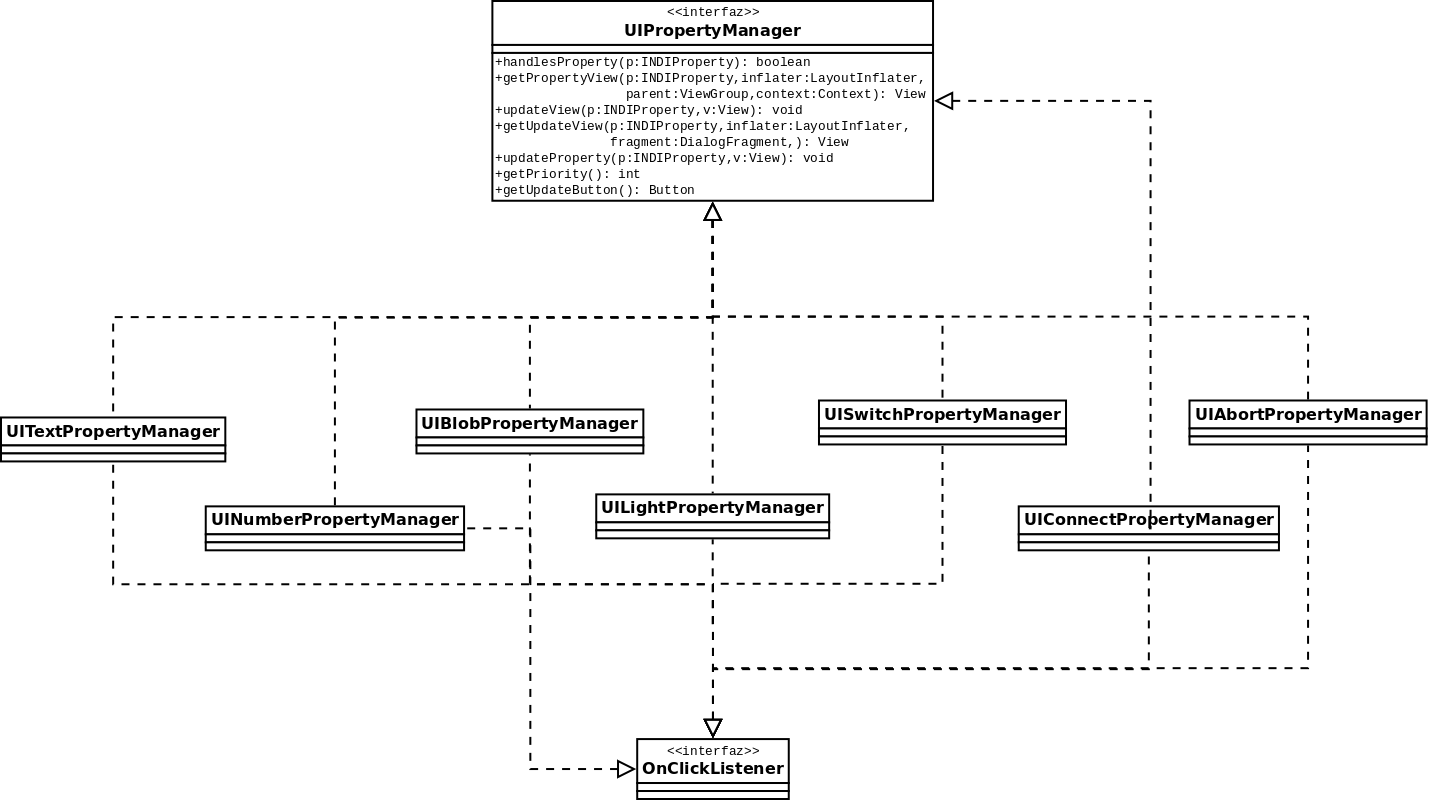
\includegraphics[width=1\textwidth]{../images/manager_ui.png}
  \caption{Diagrama de clases asociadas a los manejadores de propiedades}
  \label{fig:diag_manager_ui}
  \end{center}
\end{figure}

\newpage
\subsection{Diseño de las clases manejadoras de dispositivos}

Finalmente, necesitamos manejar y decidir como mostramos una propiedad y sus elementos. Para implementar esta funcionalidad se ha optado por utilizar los elementos visuales de Android \textit{tabs} que permiten mostrar vistas tabuladas. Con esto, vamos a crear una vista por defecto para cualquier dispositivo. Esta vista es la utilizada en las secciones anteriores: \textit{las listas expandibles de android}.

\bigskip
En la figura \ref{fig:diag_manager_ui_device} podemos ver que tenemos una clase \textit{DefaultDeviceView} que se mostrará por defecto para todas los dispositivos. Este es el comportamiento normal de la aplicación

\bigskip
Siguiente con el objetivo principal de facilitar la extensibilidad para añadir nuevas vistas de dispositivo, se ha diseñado una clase abstracta, \textit{DeviceView}, para facilitar la creación de nuevas vistas. Solo tenemos que crear una clase que herede de esta clase abstracta e implementar los métodos. Al ser una clase que hereda de \textit{Fragment}, dentro de ella tenemos libertad para mostrar las propiedades del dispositivo para personalizarlo. Cada nueva vista sería una tabulación más en la vista tabulada.


\bigskip
\begin{figure}[!ht]
  \begin{center}
  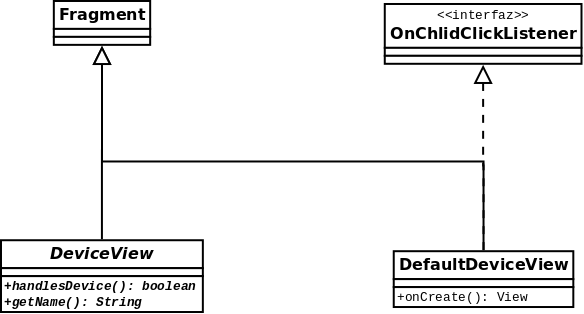
\includegraphics[width=1\textwidth]{../images/device_ui.png}
  \caption{Diagrama de clases asociadas a los manejadores de dispositivos}
  \label{fig:diag_manager_ui_device}
  \end{center}
\end{figure}


\bigskip
\section{Diseño de las interfaces de usuario}

Las interfaces de usuario deben ser objeto de un cuidadoso diseño dado que estamos construyendo una aplicación móvil, y el exito dependerá en gran medida de una buena interfaz de usuario que sea útil, clara y fácil de usar.

\bigskip
Para poder abordar mejor el diseño, se han separados las interfaces en los siguientes grupos:

\begin{itemize}
  \item \textbf{Interfaz principal de la aplicación.}
  \item \textbf{Interfaz para listar las propiedades.}
  \item \textbf{Interfaz de propiedad.}
  \item \textbf{Interfaz de dialogos}
  \item \textbf{Interfaz del log}
  \item \textbf{Interfaz de los ajustes}
\end{itemize}

\bigskip
\subsection{}


\bigskip
\section{Mecanismo de adición de vistas}